\documentclass{article}
\usepackage[utf8]{inputenc}
\usepackage[fontsize=13pt]{scrextend}
\usepackage{geometry}
\usepackage{multicol}
\usepackage{lmodern} % For scalable Computer Modern fonts
\usepackage[T1]{fontenc} % Ensures proper font encoding
\usepackage{color}
\usepackage{helvet}  % For changing fonts

\usepackage{soul}  % For highlighting

\geometry{
  a4paper,
  left=25mm,
  right=25mm,
  top=25mm,
  bottom=25mm,
  heightrounded,
}
\usepackage[T1]{fontenc}
\usepackage{amsmath}
\usepackage{amsfonts}
\usepackage{amssymb}
\usepackage{graphicx}
\usepackage{tabularx}
\usepackage{lastpage}
\usepackage{xcolor}
\usepackage{tikz}
\usepackage{pgfplots}
\usepackage{hyperref}
\usepackage{listings}
\usepackage{booktabs}
\usepackage{tabularray}
\usepackage{multirow}
\usepackage{float}
\usepackage{lastpage}
\usepackage{tcolorbox}
\usepackage{titlesec}

\usepackage{etoolbox}

\makeatletter
\patchcmd{\@zfancyhead}{\fancy@reset}{\f@nch@reset}{}{}
\patchcmd{\@set@em@up}{\f@ncyolh}{\f@nch@olh}{}{}
\patchcmd{\@set@em@up}{\f@ncyolh}{\f@nch@olh}{}{}
\patchcmd{\@set@em@up}{\f@ncyorh}{\f@nch@orh}{}{}
\makeatother



\usepackage{lastpage} % Required to determine the last page number for the footer

\usepackage{graphicx} % Required to insert images

\setlength\parindent{0pt} % Removes all indentation from paragraphs

\usepackage[most]{tcolorbox} % Required for boxes that split across pages

\usepackage{booktabs} % Required for better horizontal rules in tables

\usepackage{listings} % Required for insertion of code

\usepackage{etoolbox} % Required for if statements

%----------------------------------------------------------------------------------------
%	MARGINS
%----------------------------------------------------------------------------------------

\usepackage{geometry} % Required for adjusting page dimensions and margins

\geometry{
	paper=a4paper, % Change to letterpaper for US letter
	top=3cm, % Top margin
	bottom=3cm, % Bottom margin
	left=2.5cm, % Left margin
	right=2.5cm, % Right margin
	headheight=14pt, % Header height
	footskip=1.4cm, % Space from the bottom margin to the baseline of the footer
	headsep=1.2cm, % Space from the top margin to the baseline of the header
	%showframe, % Uncomment to show how the type block is set on the page
}

%----------------------------------------------------------------------------------------
%	FONT
%----------------------------------------------------------------------------------------

\usepackage[utf8]{inputenc} % Required for inputting international characters
\usepackage[T1]{fontenc} % Output font encoding for international characters

\usepackage[sfdefault,light]{roboto} % Use the Roboto font

%----------------------------------------------------------------------------------------
%	HEADERS AND FOOTERS
%----------------------------------------------------------------------------------------

\usepackage{fancyhdr} % Required for customising headers and footers

\pagestyle{fancy} % Enable custom headers and footers

\lhead{\small\assignmentClass\ifdef{\assignmentClassInstructor}{\ (\assignmentClassInstructor):}{}\ \assignmentTitle} % Left header; output the instructor in brackets if one was set
\chead{} % Centre header
\rhead{\small\ifdef{\assignmentAuthorName}{\assignmentAuthorName}{\ifdef{\assignmentDueDate}{Due\ \assignmentDueDate}{}}} % Right header; output the author name if one was set, otherwise the due date if that was set

\lfoot{} % Left footer
\cfoot{\small Page\ \thepage\ of\ \pageref{LastPage}} % Centre footer
\rfoot{} % Right footer

\renewcommand\headrulewidth{0.5pt} % Thickness of the header rule

%----------------------------------------------------------------------------------------
%	MODIFY SECTION STYLES
%----------------------------------------------------------------------------------------

\usepackage{titlesec} % Required for modifying sections
\usepackage{longtable}
%------------------------------------------------
% Section

\titleformat
{\section} % Section type being modified
[block] % Shape type, can be: hang, block, display, runin, leftmargin, rightmargin, drop, wrap, frame
{\Large\bfseries} % Format of the whole section
{\assignmentQuestionName~\thesection} % Format of the section label
{6pt} % Space between the title and label
{} % Code before the label

\titlespacing{\section}{0pt}{0.5\baselineskip}{0.5\baselineskip} % Spacing around section titles, the order is: left, before and after

%------------------------------------------------
% Subsection

\titleformat
{\subsection} % Section type being modified
[block] % Shape type, can be: hang, block, display, runin, leftmargin, rightmargin, drop, wrap, frame
{\itshape} % Format of the whole section
{(\alph{subsection})} % Format of the section label
{4pt} % Space between the title and label
{} % Code before the label

\titlespacing{\subsection}{0pt}{0.5\baselineskip}{0.5\baselineskip} % Spacing around section titles, the order is: left, before and after

\renewcommand\thesubsection{(\alph{subsection})}

%----------------------------------------------------------------------------------------
%	CUSTOM QUESTION COMMANDS/ENVIRONMENTS
%----------------------------------------------------------------------------------------

% Environment to be used for each question in the assignment
\newenvironment{question}{
	\vspace{0.5\baselineskip} % Whitespace before the question
	\section{} % Blank section title (e.g. just Question 2)
	\lfoot{\small\itshape\assignmentQuestionName~\thesection~continued on next page\ldots} % Set the left footer to state the question continues on the next page, this is reset to nothing if it doesn't (below)
}{
	\lfoot{} % Reset the left footer to nothing if the current question does not continue on the next page
}

%------------------------------------------------

% Environment for subquestions, takes 1 argument - the name of the section
\newenvironment{subquestion}[1]{
	\subsection{#1}
}{
}

%------------------------------------------------

% Command to print a question sentence
\newcommand{\questiontext}[1]{
	\textbf{#1}
	\vspace{0.5\baselineskip} % Whitespace afterwards
}

%------------------------------------------------

% Command to print a box that breaks across pages with the question answer
\newcommand{\answer}[1]{
	\begin{tcolorbox}[breakable, enhanced]
		#1
	\end{tcolorbox}
}

%------------------------------------------------

% Command to print a box that breaks across pages with the space for a student to answer
\newcommand{\answerbox}[1]{
	\begin{tcolorbox}[breakable, enhanced]
		\vphantom{L}\vspace{\numexpr #1-1\relax\baselineskip} % \vphantom{L} to provide a typesetting strut with a height for the line, \numexpr to subtract user input by 1 to make it 0-based as this command is
	\end{tcolorbox}
}

%------------------------------------------------

% Command to print an assignment section title to split an assignment into major parts
\newcommand{\assignmentSection}[1]{
	{
		\centering % Centre the section title
		\vspace{2\baselineskip} % Whitespace before the entire section title
		
		\rule{0.8\textwidth}{0.5pt} % Horizontal rule
		
		\vspace{0.75\baselineskip} % Whitespace before the section title
		{\LARGE \MakeUppercase{#1}} % Section title, forced to be uppercase
		
		\rule{0.8\textwidth}{0.5pt} % Horizontal rule
		
		\vspace{\baselineskip} % Whitespace after the entire section title
	}
}

%----------------------------------------------------------------------------------------
%	TITLE PAGE
%----------------------------------------------------------------------------------------

\author{\textbf{\assignmentAuthorName}} % Set the default title page author field
\date{} % Don't use the default title page date field

\title{
	\thispagestyle{empty} % Suppress headers and footers
	\vspace{0.2\textheight} % Whitespace before the title
	\textbf{\assignmentClass:\ \assignmentTitle}\\[-4pt]
	\ifdef{\assignmentDueDate}{{\small Due\ on\ \assignmentDueDate}\\}{} % If a due date is supplied, output it
	\ifdef{\assignmentClassInstructor}{{\large \textit{\assignmentClassInstructor}}}{} % If an instructor is supplied, output it
	\vspace{0.32\textheight} % Whitespace before the author name
}


\pgfplotsset{compat=newest}

% Colors from structure.tex
\definecolor{secondaryColor}{RGB}{0,0,0}
\definecolor{accentColor1}{RGB}{255,87,34}
\definecolor{accentColor3}{RGB}{63,81,181}
\definecolor{textColor}{RGB}{33,33,33}
\definecolor{primaryColor}{RGB}{34, 45, 101}
\definecolor{accentColor2}{RGB}{46, 117, 182}
\definecolor{backgroundColor}{RGB}{245, 245, 245}

% Redefine section format to include color
\titleformat{\section}
  {\color{primaryColor}\Large\bfseries}
  % {\color{primaryColor}\assignmentQuestionName~\thesection}
  {6pt}
  {}

\newcommand{\highlight}[1]{\textsf{\textbf{#1}}}  % For highlighting key terms in sans-serif bold


% Redefine subsection format to include color
\titleformat{\subsection}
  {\color{secondaryColor}\itshape}
  {\color{secondaryColor}(\alph{subsection})}
  {4pt}
  {}

% % Modify the question environment to include color
% \renewenvironment{question}{
%   \vspace{0.5\baselineskip}
%   \section{}
%   \lfoot{\small\itshape\color{primaryColor}\assignmentQuestionName~\thesection~continued on next page\ldots}
% }{
%   \lfoot{}
% }

% Modify the answer command to include color
\renewcommand{\answer}[1]{
  \begin{tcolorbox}[
    breakable,
    enhanced,
    colback=backgroundColor,
    colframe=primaryColor,
    coltitle=white,
    title=Answer
  ]
    #1
  \end{tcolorbox}
}

% Modify the assignmentSection command to include color
\renewcommand{\assignmentSection}[1]{
  {
    \centering
    \vspace{2\baselineskip}
    
    \color{primaryColor}\rule{0.8\textwidth}{0.5pt}
    
    \vspace{0.75\baselineskip}
    {\LARGE\color{primaryColor}\MakeUppercase{#1}}
    
    \color{primaryColor}\rule{0.8\textwidth}{0.5pt}
    
    \vspace{\baselineskip}
  }
}

% Modify headers and footers to include color
\lhead{\small\color{primaryColor}\assignmentClass\ifdef{\assignmentClassInstructor}{\ (\assignmentClassInstructor):}{Ayush Kumar Mishra}\ \assignmentTitle}
\rhead{\small\color{secondaryColor}\ifdef{\assignmentAuthorName}{\assignmentAuthorName}{\ifdef{\assignmentDueDate}{Due\ \assignmentDueDate}{}}}
\cfoot{\small\color{primaryColor}Page\ \thepage\ of\ \pageref{LastPage}}

\renewcommand\headrulewidth{0.5pt}
\renewcommand{\headrule}{\hbox to\headwidth{\color{primaryColor}\leaders\hrule height \headrulewidth\hfill}}

\hypersetup{
    colorlinks=true,
    linkcolor=primaryColor,
    filecolor=accentColor1,      
    urlcolor=accentColor3,
    pdftitle={Advanced EDA of Video Text Dataset},
    pdfpagemode=FullScreen,
}

\title{\textcolor{primaryColor}{\Huge\textbf{Advanced EDA of Video Text Dataset}}}
\author{\textcolor{secondaryColor}{\Large Data Science Team}}
\date{\textcolor{secondaryColor}{\today}}

\begin{document}

\maketitle

\newpage
\section*{Dashboard}
\begin{center}
\vspace{2in}
    {\Huge  For seeing all the code live interactively, \\
    \vspace{2in}
    Visit  \href{https://eda-analysis-iby-0.streamlit.app/}{Dashboard}}\\
    
    \vspace{0.7in}
   \textbf{ \href{https://eda-analysis-iby-0.streamlit.app/}{https://eda-analysis-iby-0.streamlit.app/}}
\end{center}

\newpage
\tableofcontents

\newpage
\section{Introduction}
This document presents an extensive Exploratory Data Analysis (EDA) of a video text dataset, focusing on emotional and communication attributes of students.

\section{Data Overview}

\subsection{Emotion Data Overview}
\textbf{emotion\_data:} This dataset contains the following columns. We can inspect the first few rows using \textit{emotion\_df.head()}.
\vspace{0.2in}
\begin{tcolorbox}[colback=backgroundColor, colframe==accentColor2, title=Emotion Data Sample, fonttitle=\bfseries]
This is a sample of emotion data.
\noindent \textbf{Description:} This dataset represents the emotions detected at each timestamp of the video, along with the dominant emotion for each image sequence.
\\
\resizebox{\textwidth}{!}{
\begin{tabular}{L{2.5cm} cccccccl}
\toprule
\textbf{Image Seq} & \textbf{Angry} & \textbf{Disgust} & \textbf{Fear} & \textbf{Happy} & \textbf{Sad} & \textbf{Surprise} & \textbf{Neutral} & \textbf{Dominant Emotion} \\
\midrule
0 & 4.32 & 0.00 & 2.88 & 1.65 & 2.78 & 0.60 & 87.77 & Neutral \\
1 & 53.23 & 2.98 & 12.74 & 1.52 & 1.05 & 27.22 & 1.26 & Angry \\
2 & 8.80 & 0.03 & 2.97 & 16.83 & 39.88 & 0.28 & 31.21 & Sad \\
3 & 9.45 & 0.11 & 1.55 & 20.93 & 3.50 & 0.91 & 63.54 & Neutral \\
4 & 56.00 & 0.00 & 0.16 & 5.58 & 0.20 & 12.81 & 25.25 & Angry \\
\bottomrule
\end{tabular}
}
\end{tcolorbox}

\subsection{Structure of Gaze Data}
\begin{tcolorbox}[colback=backgroundColor, colframe=accentColor2, title=Gaze Data Structure, fonttitle=\bfseries]
\begin{tabular}{p{2.5cm} ccc}
\toprule
\textbf{Image Seq} & \textbf{Gaze} & \textbf{Blink} & \textbf{Eye Offset} \\
\midrule
1 & 1 & 0 & 6.23 \\
2 & 1 & 0 & 22.73 \\
3 & 1 & 0 & 2.57 \\
4 & 1 & 0 & 21.11 \\
5 & 1 & 0 & 1.85 \\
\bottomrule
\end{tabular}
\end{tcolorbox}


\vspace{0.5in}

% Transcript Data Section
% \section{Transcript Data Analysis}
\subsection{Transcript Data Sample}
\begin{tcolorbox}[
colback=backgroundColor,
colframe=accentColor2,
title=Transcript Data Sample,
fonttitle=\bfseries
]
\resizebox{\textwidth}{!}{
\begin{tblr}{
colspec = {lcccccccc},
row{1} = {font=\bfseries},
hlines,
vlines,
stretch = 1
}
\textbf{id} & \textbf{text} & \textbf{tokens} & \textbf{positive} & \textbf{negative} & \textbf{neutral} & \textbf{confident} & \textbf{hesitant} & \textbf{concise} & \textbf{enthusiastic} & \textbf{speech\_speed} \\
0 & Hello, I am J & [50364, 24] & 0.5803 & 0.1523 & 0.2675 & 0.8467 & 0.8457 & 0.6358 & 0.6478 & 2.518 \\
1 & IIM Coikode. & [50642, 28] & 0.5503 & 0.1893 & 0.2604 & 0.6793 & 0.7337 & 0.5441 & 0.4174 & 3.2178 \\
2 & Technology & [50844, 15] & 0.6399 & 0.1111 & 0.2490 & 0.9027 & 0.8346 & 0.7159 & 0.7001 & 2.8689 \\
3 & of three yea & [51088, 29] & 0.4419 & 0.3992 & 0.1589 & 0.7743 & 0.8130 & 0.5225 & 0.2799 & 3.750 \\
4 & as a medical & [51288, 38] & 0.2363 & 0.5320 & 0.2317 & 0.2860 & 0.5614 & 0.3344 & 0.1973 & 3.5417 \\
\end{tblr}
}
\end{tcolorbox}




\subsection{Basic Statistics}
\begin{tcolorbox}[
colback=backgroundColor,
colframe=accentColor2,
title=Basic Statistics,
fonttitle=\bfseries
]
\resizebox{\textwidth}{!}{
\begin{tblr}{
colspec = {lcccccccccccc},
row{1} = {font=\bfseries},
hlines,
vlines,
stretch = 1
}
\textbf{} & \textbf{id} & \textbf{seek} & \textbf{start} & \textbf{end} & \textbf{positive} & \textbf{negative} & \textbf{neutral} & \textbf{confident} & \textbf{hesitant} & \textbf{concise} & \textbf{enthusiastic} & \textbf{speech\_speed} \\
count & 18 & 18 & 18 & 18 & 18 & 18 & 18 & 18 & 18 & 18 & 18 & 18 \\
mean & 8.5 & 3,009.33 & 41.0022 & 45.9311 & 0.7092 & 0.1412 & 0.1496 & 0.7338 & 0.4852 & 0.4294 & 0.4665 & 3.1138 \\
std & 5.3385 & 2,598.47 & 26.117 & 26.2949 & 0.2073 & 0.1549 & 0.0810 & 0.2083 & 0.2608 & 0.2726 & 0.2863 & 0.600 \\
min & 0 & 0 & 0 & 5.56 & 0.2363 & 0.0050 & 0.0146 & 0.2860 & 0.0084 & 0.0128 & 0.0886 & 2.0349 \\
25\% & 4.25 & 0 & 19.68 & 24.4 & 0.5879 & 0.0433 & 0.0829 & 0.5769 & 0.3429 & 0.2808 & 0.2114 & 2.6057 \\
50\% & 8.5 & 2,776 & 40.56 & 46.64 & 0.7397 & 0.0804 & 0.1557 & 0.7899 & 0.4078 & 0.4415 & 0.4189 & 3.1342 \\
75\% & 12.75 & 5,336 & 62.42 & 66.66 & 0.8701 & 0.1602 & 0.2246 & 0.8986 & 0.7108 & 0.6129 & 0.6870 & 3.5897 \\
max & 17 & 8,272 & 82.72 & 88.72 & 0.9804 & 0.5320 & 0.2675 & 0.9809 & 0.8457 & 0.9197 & 0.9903 & 4.1667 \\
\end{tblr}
}
\end{tcolorbox}




% Removing irrelevant columns for a cleaner view
Note: In the transcript data, the columns \textit{text}, \textit{tokens}, \textit{temperature}, \textit{avg\_logprob}, \textit{compression\_ratio}, and \textit{no\_speech\_prob} are removed for simplification.



\section{Data Preprocessing}
\begin{tcolorbox}[colback=teal!5!white,colframe=teal!75!black,title= Steps for Data preprocessing]
\textbf{The following steps were performed to preprocess the data before conducting any Exploratory Data Analysis (EDA):}

\begin{itemize}
    \item \textbf{Handling Missing Values:} Replaced missing or null values using techniques such as mean, median, or mode imputation based on the feature type.
    \item \textbf{Encoding Categorical Features:} Converted categorical variables into numeric form using label encoding or one-hot encoding.
    \item \textbf{Scaling and Normalization:} Applied standard scaling or min-max normalization to ensure that features with different units or ranges do not dominate the model's learning process.
    % Add other preprocessing steps from the original document
\end{itemize}
\end{tcolorbox}



\section{Data Preparation and Integration}

So, the data is spread across three different CSV files, and what I need to do is pull out key features from all of them to create a single, clean DataFrame.

\noindent\sffamily
First off, I’m going to take the \highlight{dominant emotions} for each student across the entire video. To do this, I’ll average the dominant emotions over every frame and then store them as \highlight{dominant\_emotion\_top\_1} and \highlight{dominant\_emotion\_top\_2}. These two values will give us a quick idea of the main emotional tones for each student.

\begin{multicols}{2}

\begin{enumerate}
    \item First, I'll \highlight{extract and compute the average values} from the \highlight{transcript data}. This is important because we need to analyze how students behave by looking at things like \highlight{positivity}, \highlight{negativity}, and \highlight{speech speed}. By averaging these features across their complete transcript, I can see overall patterns, like how often they seem confident or hesitant.
    
    \item Then, I’ll \highlight{store these averages in a list of DataFrames}. The reason for this is to keep track of each student’s data separately at first. This way, when I combine them later, it’s easier to manage and analyze.
    
    \item After that, I’ll \highlight{combine all the averages into one final DataFrame}. This step is key because it gives me a \highlight{well-organized dataset} where I can quickly compare each student’s average speech features. So, up to here, the \highlight{transcript part} is done.
    
    \item Next, I’ll \highlight{extract the dominant emotions} from the \highlight{emotion data}. The goal here is to capture the emotional tone of each student by identifying the \highlight{most frequent emotions}—whether they're happy, sad, or something else. This adds more depth to the average speech features we just looked at.
    
    \item Once I have the dominant emotions, I’ll \highlight{store the top two} for each student. This is important because it gives us a quick snapshot of their \highlight{emotional profile} during speech, covering both the primary and secondary emotions. It’s like getting the full emotional picture.
    
    \item I’ll then \highlight{create a DataFrame} to hold all these dominant emotions. Having this in a separate DataFrame makes it easy to \highlight{merge with the average speech features}, so I can analyze everything together in one place.
    
    \item Now, I’ll \highlight{merge the average features DataFrame with the dominant emotions DataFrame}. This combination gives me a comprehensive dataset, mixing both the \highlight{quantitative data} (like positivity and speech speed) with more \highlight{qualitative data} (like emotions), which lets me dig deeper into how students' behavior and emotions interact.
    
    \item Finally, I’ll \highlight{display the complete DataFrame}. This final view will give a \highlight{clear overview} of each student's \highlight{speech patterns} and \highlight{emotional tendencies}, which will help understand their \highlight{communication behavior} better and could guide future feedback or interventions.
\end{enumerate}

\end{multicols}
\newpage

So this is my new DATAFRAME , Let's call it \textsc{final_df}
\begin{center}
    
\includegraphics[width=1/columnwidth]{}
\end{center}


\section{Advanced Analysis}
\begin{center}
    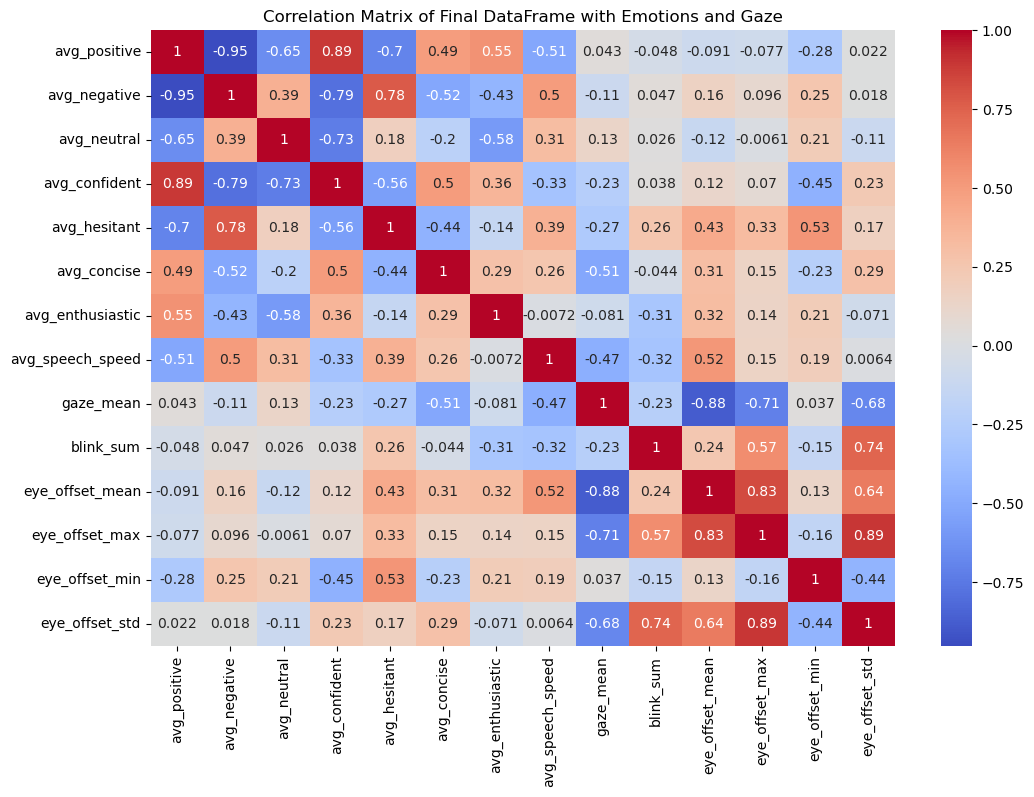
\includegraphics[width=1\columnwidth]{images/corr_matrix_of_final_data.png}
    \caption{}
    \label{fig:enter-label}
\end{center}


\begin{tcolorbox}[colback=cyan!5!white,colframe=cyan!75!black,title= Insights from the correlation matrix]
\textbf{Focusing on this image, We can conclude :}
\begin{itemize}
    \item \textbf{avg\_positve and avg\_confident is highly correlated as red means they are correlated.}
    \item \textbf{avg\_hesitant and avg\_negative is also correlated as they are blue and their correlation score is 0.77(quite high) .}
    \item \textbf{avg\_enthusiastic and avg\_confident is also correlated though not as high as avg\_positive and avg\_confident.}
    \item \textbf{avg\_negative and avg\_confident is highly uncorrelated and their correlation score is -0.73(quite high) .}
\end{itemize}

\textbf{In this way, we can see the correlation between the features like which features are dependent or which are not.}
 From this we can if a student whose text content score is positive, then he/she is more likely more confident and enthusiastic
 in comparison to the student whose text content score is negative. This fact will help in further analysis.\\ 
    \vspace{0.2in}

\end{tcolorbox}


Distribution plots were generated for various features to understand their spread and central tendencies. For example:

\begin{figure}[H]
    \centering
    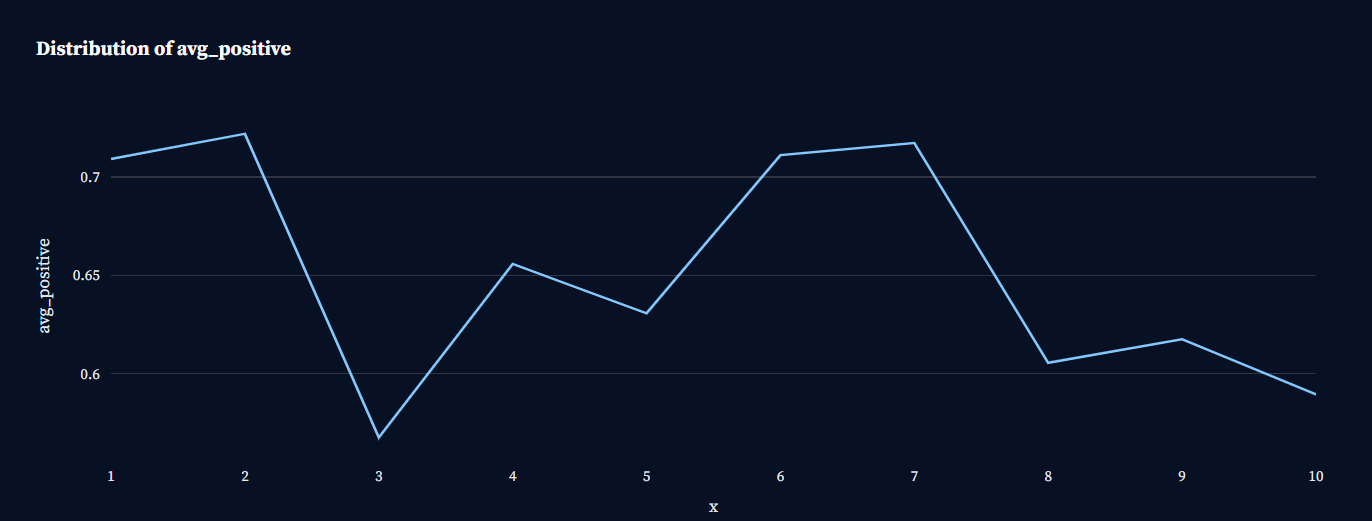
\includegraphics[width=0.8\textwidth]{images/avg_positve_distribution.png}
    \caption{Distribution of avg\_positive scores}
    \label{fig:avg_positive_distribution}
\end{figure}


\begin{figure}[H]
    \centering
    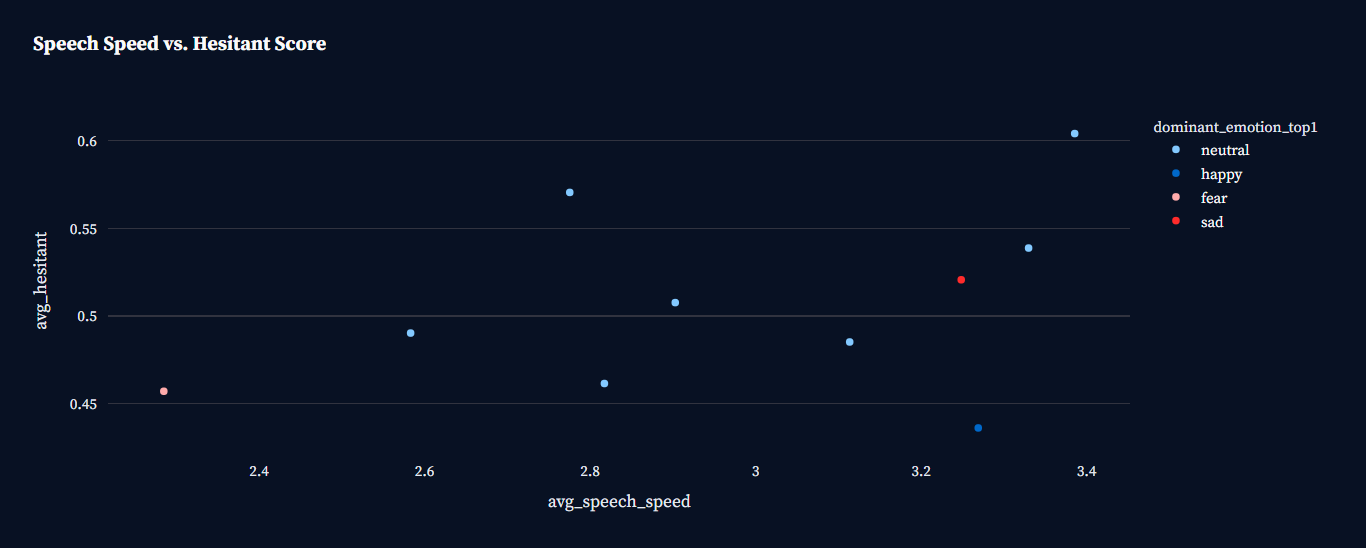
\includegraphics[width=0.8\textwidth]{images/speech_speed_vs_hesitant.png}
    \caption{Speech Speed vs. Hesitant Scores}
    \label{fig:speech_speed_vs_hesitant}
\end{figure}


\subsection{Communication Skills Analysis}
\begin{itemize}
    \item \textbf{First}, I will investigate the relationship between \textbf{conciseness} and \textbf{enthusiasm} of the students.\\ 
    For this, I am plotting a joint plot between avg\_concise and avg\_enthusiastic. From the plot, we can see that there is a positive correlation between the two features.\\
    
    This indicates that students who are more concise in their speech are also more enthusiastic.
    % make columns for images first one this join plot and other scatter plot between avg_speech_speed and avg_hesitant

    
    \begin{center}
        \begin{minipage}{0.45\textwidth}
        \centering
        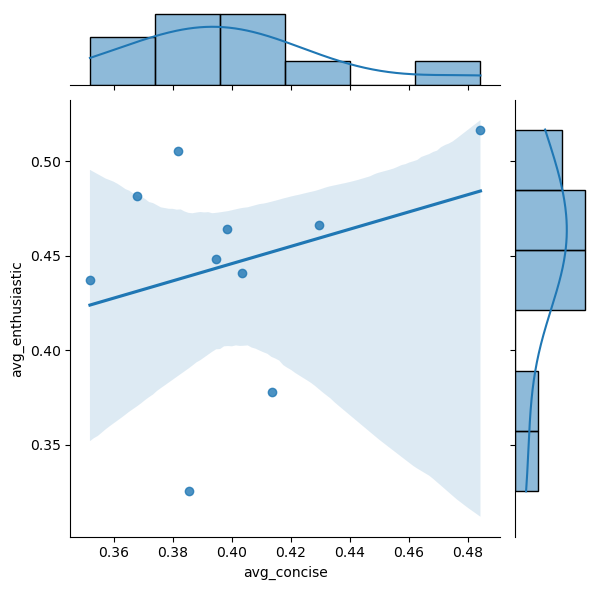
\includegraphics[width=\textwidth]{images/joinplot_between_avg_enthusiatic_and_avg_concise.png}
        \caption{Joint plot between avg\_enthusiastic and avg\_concise.}
    \end{minipage}\hfill
    \begin{minipage}{0.45\textwidth}
        \centering
        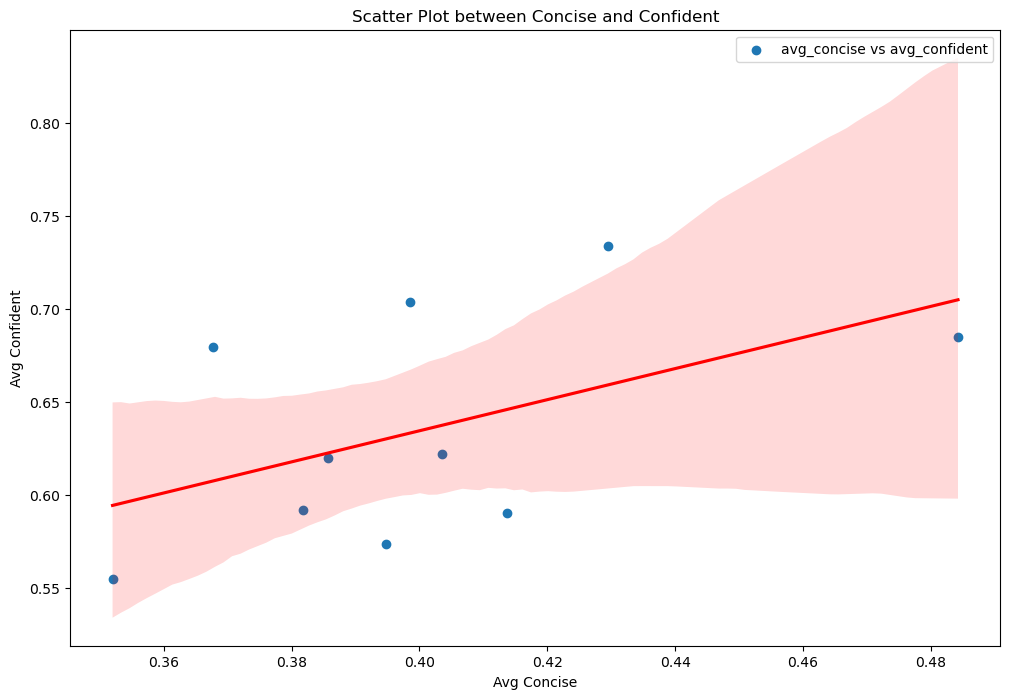
\includegraphics[width=\textwidth]{images/concise_confi.png}
        \caption{Scatter plot between avg\_speech\_speed and avg\_hesitant.}
    \end{minipage}
    \caption{Comparison of conciseness vs enthusiasm and confidence.}
    \end{center}

    \item \textbf{Communication} skill is also dependent on the \textbf{speed of speech}. To analyze this, I am plotting a scatter plot between avg\_speech\_speed and avg\_hesitant.\\
    
    The plot reveals a negative correlation between these two features, meaning that students who speak faster are less hesitant in their speech.
    \begin{center}
        \begin{minipage}{0.45\textwidth}
            \centering
            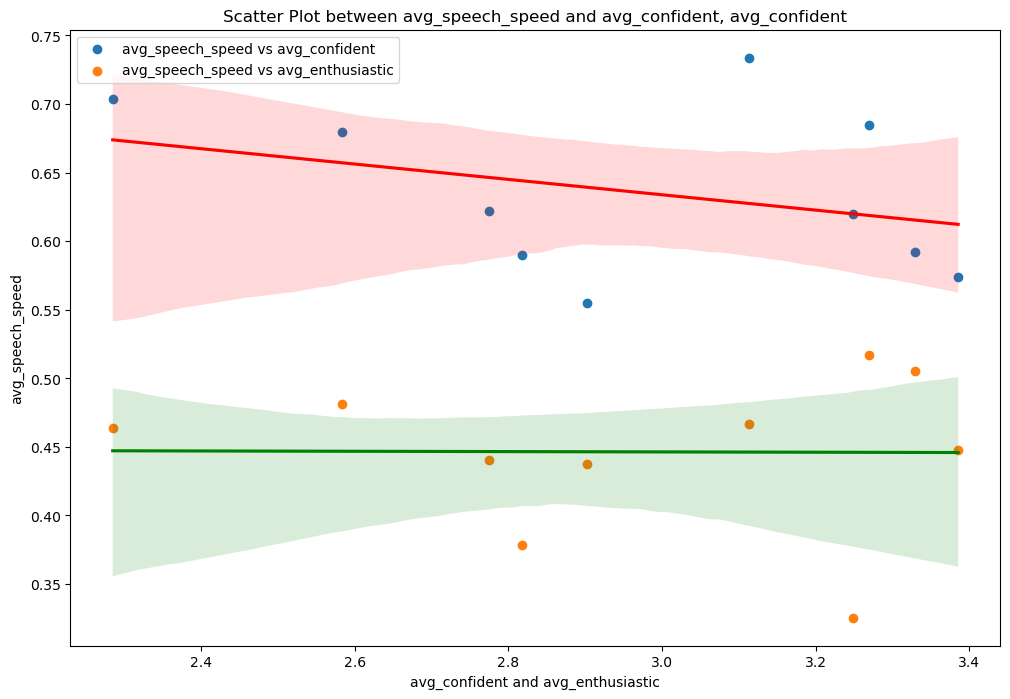
\includegraphics[width=\textwidth]{images/speech_confi.png}
            \caption{Scatter plot between avg\_speech\_speed and avg\_confidence.}
        \end{minipage}\hfill
        \begin{minipage}{0.45\textwidth}
            \centering
            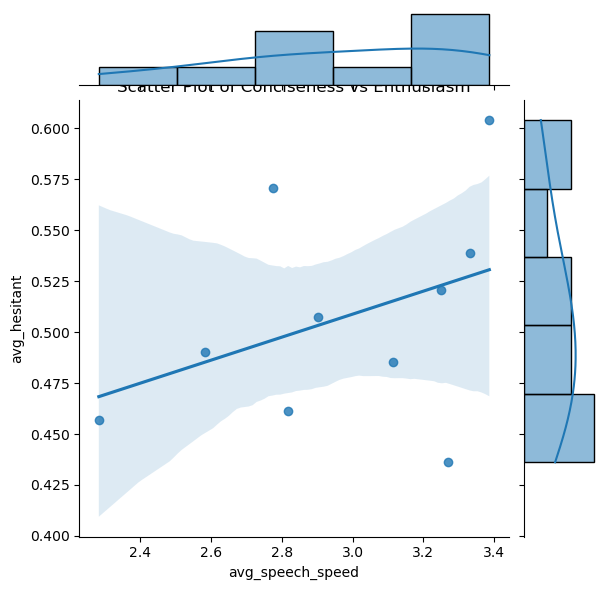
\includegraphics[width=\textwidth]{images/avg_speech_speed_vs_avg_hesitant.png}
            \caption{Scatter plot between avg\_speech\_speed and avg\_hesitant.}
        \end{minipage}{0.45\textwidth}
         \end{center}

    \item \textbf{Text} content scores (positive, negative, neutral) are also crucial in communication skills. Therefore, I will analyze the relationship between \textbf{positivity} and \textbf{confidence} of the students.\\ 

    
    For this, I am plotting a scatter plot between avg\_positive and avg\_confident. The plot shows a positive correlation between these features, indicating that students with a more positive text content score are also more confident in their speech.
    \begin{center}
        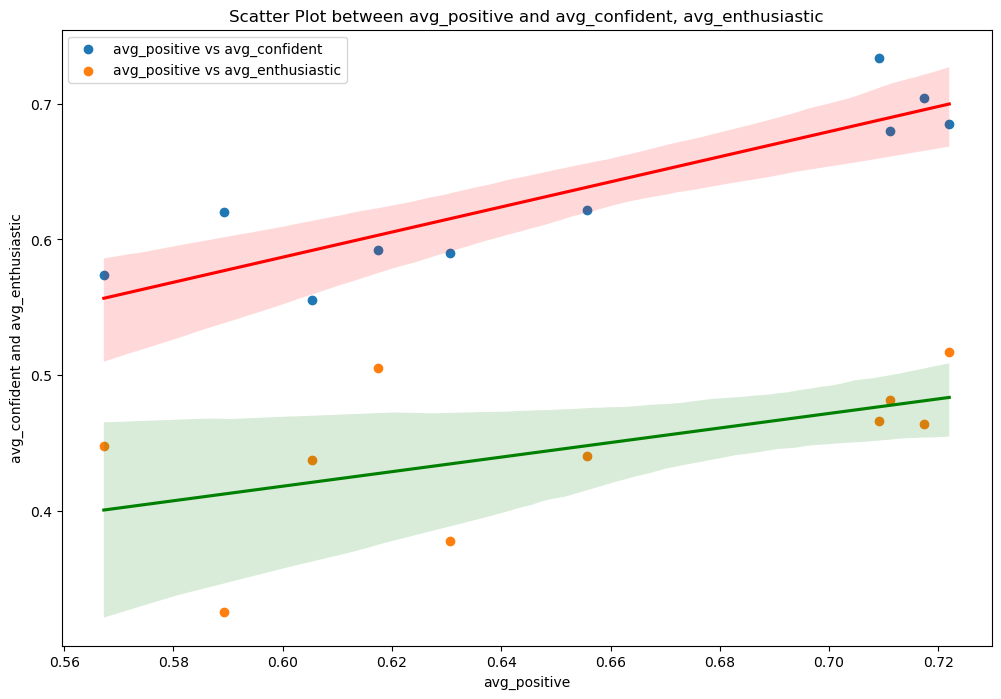
\includegraphics[width=1\columnwidth]{images/scatter_plot_avgPositve_and_avg_confident_avg_enthusiatist.png}
    \end{center}
    From this graph, we can clearly see the linear relation between avg\_positive vs avg\_confident and avg\_positive vs avg\_enthusiastic. 

    \item \textbf{Additionally}, the relationship between avg\_negative and avg\_confident is also linear but in the opposite direction.\\  

    
    
    This implies that students with a more negative text content score tend to be less confident and enthusiastic. 

    \begin{center}
        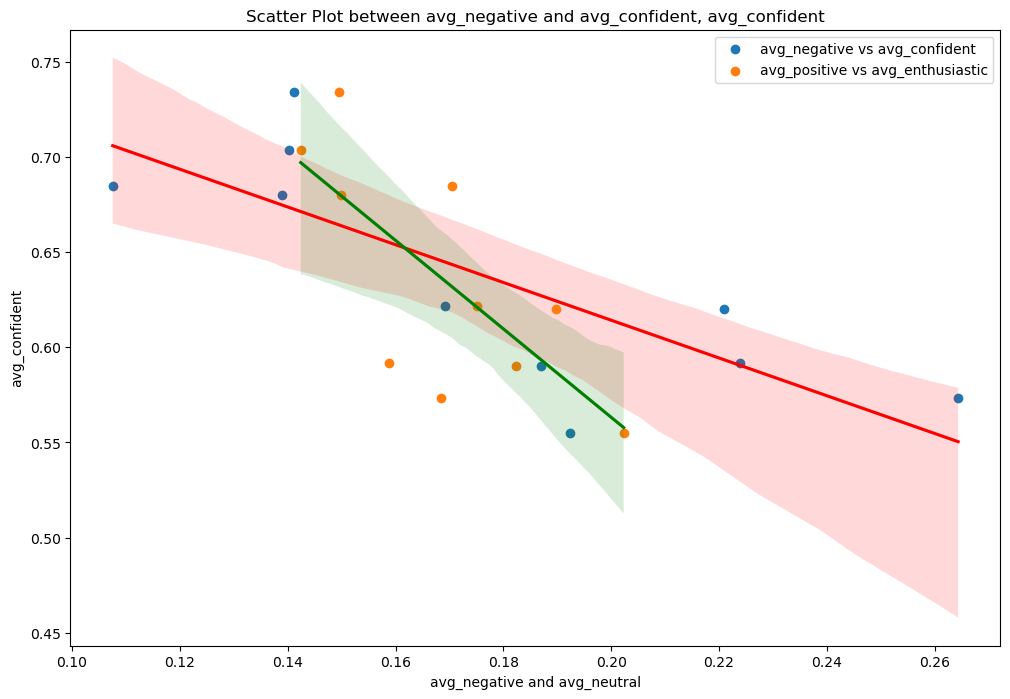
\includegraphics[width=1\columnwidth]{images/avgNeg_conf.png}
    \end{center}
    \begin{center}
      \begin{tikzpicture}[scale=0.9, every node/.style={scale=0.9}]
      
          % Positive Correlation
          \begin{scope}[yshift=6cm]
              \draw[->, thick] (0,0) -- (4,2) node[midway, above right] {\textbf{Positive Correlation}};
              \draw[->, thick] (0,0) -- (4,0) node[midway, below] {Positive Text Score};
              \draw[->, thick] (0,0) -- (0,2) node[midway, left] {Confidence/Enthusiasm};
          
              % Add labels for the positive case
              \node[text width=3cm, align=left] at (5, 1) 
          \end{scope}
      
          % Neutral Correlation
          \begin{scope}[yshift=3cm]
              \draw[->, thick, color=blue] (0,0) -- (4,0) node[midway, below] {Neutral Text Score};
              \draw[->, thick, color=blue] (0,0) -- (0,2) node[midway, left] {Confidence/Enthusiasm};
               \draw[->, thick, color=red] (0,2) -- (4,0) node[midway, below right] {\textbf{Negative Correlation}};
          
              % Add labels for the neutral case
              \node[text width=3cm, align=left] at (5, 1) 
          \end{scope}
      
          % Negative Correlation
          \begin{scope}
              \draw[->, thick, color=red] (0,2) -- (4,0) node[midway, below right] {\textbf{Negative Correlation}};
              \draw[->, thick, color=red] (0,0) -- (4,0) node[midway, below] {Negative Text Score};
              \draw[->, thick, color=red] (0,0) -- (0,2) node[midway, left] {Confidence/Enthusiasm};
          
              % Add labels for the negative case
              \node[text width=3cm, align=left] at (5, 1) 
          \end{scope}
      
      \end{tikzpicture}
      \caption{Correlation Diagram for Text Scores with Confidence and Enthusiasm}
      \label{fig:correlation-diagram}
  \end{center}
      
    \item An interesting insight from the above graph is that avg\_neutral is also linearly related to avg\_confident and avg\_enthusiastic, but in the opposite direction. This provides new insights into how neutrality in text content affects communication skills.
    
    \item 
    \vspace{0.1in}
\end{itemize}


\subsection{Emotional State and Body Language Analysis}
% Include content about stacked area charts, emotional stability analysis, etc.

1.\textbf{Emotional Stability Analysis} \\
So, I have calculated the \textbf{emotional stability} of each student by analyzing the \textbf{variability} in their emotions throughout the video.\\  

\textbf{Emotional stability} is a key factor in understanding how well students can manage their emotions during communication.\\
This is important because it helps us understand how consistent a student is in expressing different emotions.\\

% Warning Box
\begin{tcolorbox}[colback=yellow!10!white, colframe=red!80!black, title=Warning]
Since there are 10 students and in this report, for a sample, I am showing the analysis for one student only. For other students' analyses, kindly visit \href{https://eda-analysis-iby-0.streamlit.app/}{the full report here}.
\end{tcolorbox}

\begin{center}
    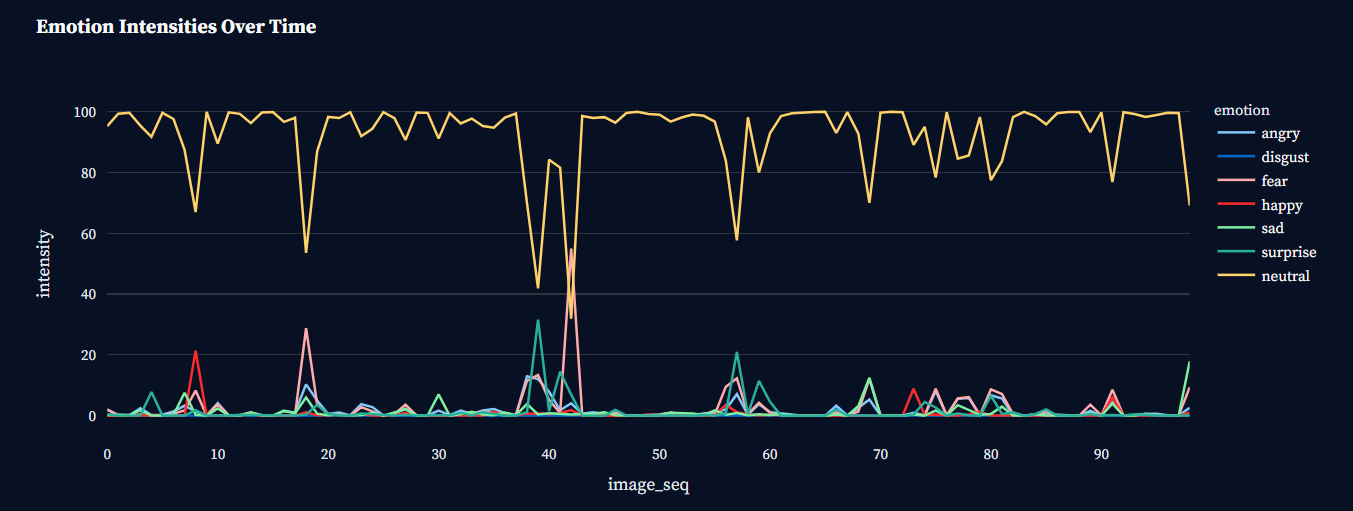
\includegraphics[width=1\columnwidth]{images/emotion_intensity_over_time.png}
\end{center}

\texttt{This student has shown a \textbf{high level of emotional stability} throughout the video, with minimal fluctuations in their emotional state.\\

There is slight moment in between where the student is showing fear and sadness.\\

This indicates that he is able to maintain a consistent emotional tone (which is neutral) during communication, which is a positive trait for effective interaction.\\
}
\normalfont

2. \textbf{Emotion Variability Analysis}\\

\textbf{Emotion variability} is another important aspect of emotional intelligence, as it reflects how well students can adapt their emotions to different situations.\\

The amount of emotions a student is showing during their speech can be an indicator of their emotional intelligence.\\

If he shows fear or sadness for a long time, then it can be a sign of less communication skills and poor body language.\\
\begin{center}
    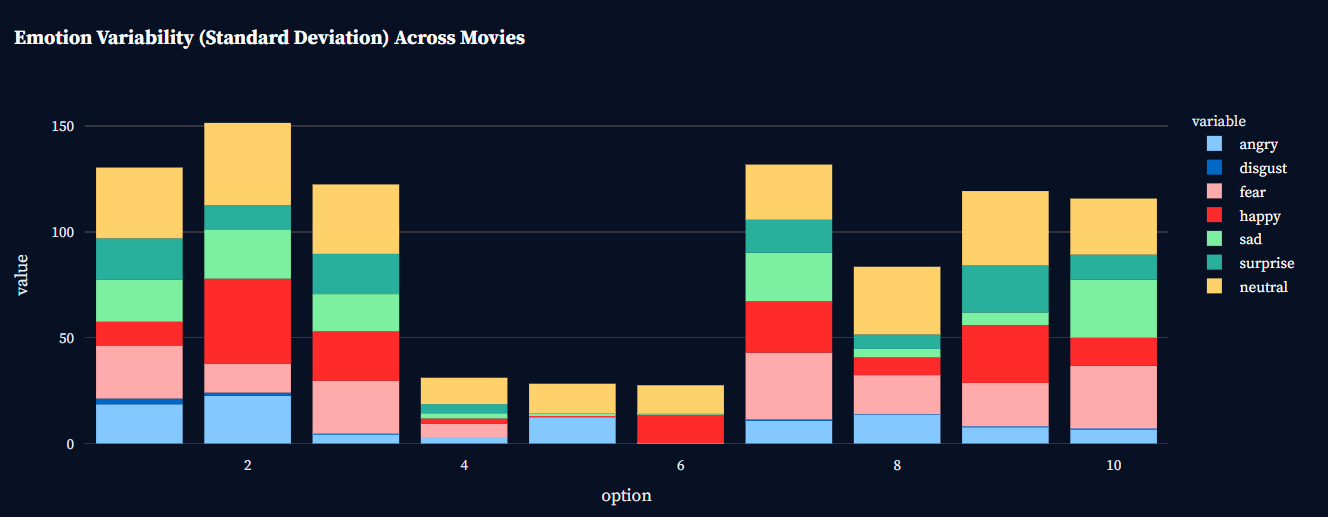
\includegraphics[width=1\columnwidth]{images/emotion_variablity.png}
\end{center}

\caption{Like in this graph, we can see that except student 5 and 6, all students are showing a good amount of variability in their emotions.}

\vspace*{0.4in}
3. \textbf{Body Language Analysis}\\
So for this, I made a new dataframe named \textsc{final-gaze\_df} which contains the gaze data of all the students.\\ 

It contains the following columns:
\begin{itemize}
    \item \texttt{movie\_id:} movie\_id
    \item \texttt{Gaze\_score:} The gaze score of the student: proportion of time the candidate spends looking at the camera..
    \item \texttt{blink\_sum:} The blink sum of the student.
    \item \texttt{eye\_offset\_std:} The eye offset standard deviation of the student.\\
    {
        \begin{enumerate}
            \item If the standard deviation (std) of the eye offset of a person in a video is too high, it suggests that the person's gaze is not stable or consistent across frames
        \end{enumerate}
    }
\end{itemize}
\vspace{0.3in}
i. \textbf{Gaze Analysis}\\
\textbf{Gaze} is an important aspect of body language that can reveal a lot about a student's focus and engagement during communication.\\

\begin{center}
    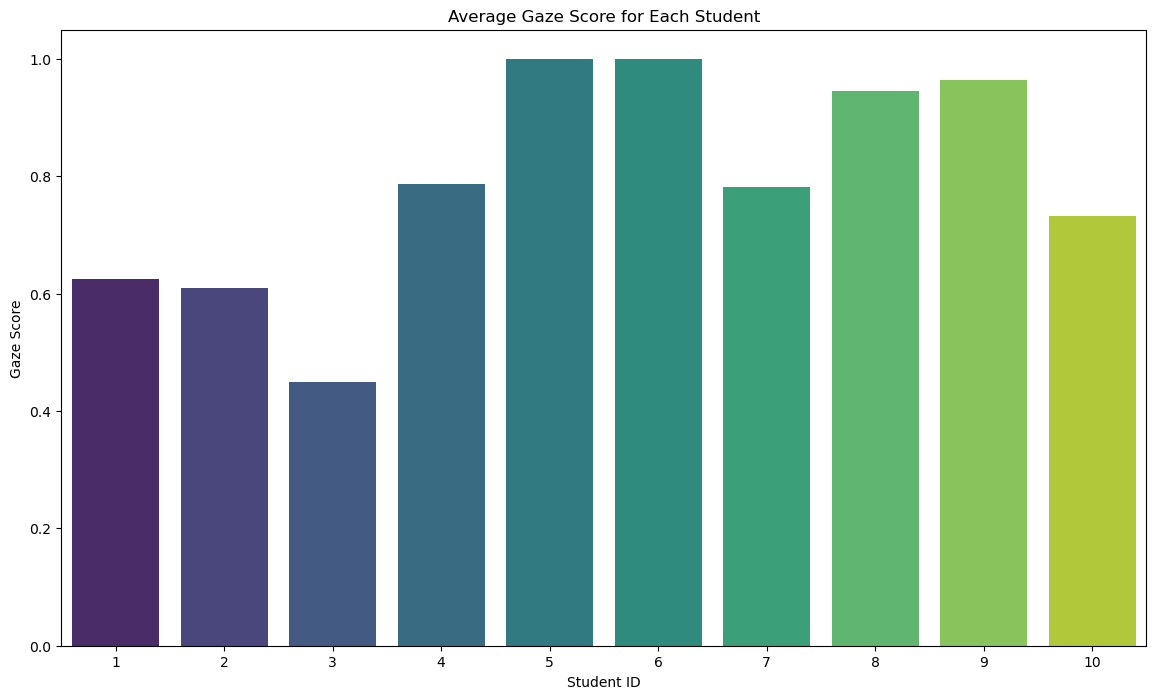
\includegraphics[width=1\columnwidth]{images/gaze_mean.png}
\end{center}

\textsc{Based on the above graph, following observations can be made:}
\begin{enumerate}
    \item Highly Engaged (0.85 - 1.0): Students who maintained frequent or constant eye contact with the camera.\\
    {
        In this category, Student 5.6,8,9 fall as their gaze score is above 0.85.
    }
    \item Moderately Engaged (0.7 - 0.85): Students who maintained moderate eye contact with the camera.\\
    {
        In this category, Student 4,7,10 fall as their gaze score is between 0.5 to 0.85.
    }
    \item Low Engagement (Below 0.7): Students who maintained low eye contact with the camera.\\
    {
        In this category, Student 1,2,3 fall as their gaze score is below 0.5.
    }
\end{enumerate}

ii. \textbf{Blink Analysis}\\
\textbf{Blinking} is another important aspect of body language that can indicate a student's level of comfort and confidence during communication.\\

\begin{center}
    \includegraphics[width=1\columnwidth]{images/blink_sum.png}
\end{center}

\textsc{Based on the above graph, following observations can be made:}

\subsection{Expertise Identification}
% Include content about Named Entity Recognition, frequency distribution of key terms, etc.

\subsection{Decision Support Metrics}
% Include content about composite scores for communication skills, emotional intelligence, etc.

\subsection{Comparative Analysis}
% Include content about comparing candidates if data is available

\subsection{Insights Generation}
% Include content about top strengths and weaknesses, communication style summary, etc.

\subsection{Recommendation Framework}
% Include content about scoring system and decision matrix

\subsection{Visualization Dashboard}
% Describe the comprehensive dashboard with key visualizations and metrics

\subsection{Further Investigation Points}
% Include content about specific moments to investigate and suggested follow-up questions

\section{Individual Student Analysis}
% Repeat this section for each student, similar to the original document
\subsection{Student 1}
% Add detailed analysis for Student 1

\subsection{Student 2}
% Add detailed analysis for Student 2

% ... Continue for all students

\section{Statistical Analysis}
% Include t-tests, ANOVA, and other statistical analyses from the original document

\section{Feature Importance}
% Include feature importance analysis from the original document

\section{Conclusion}
This comprehensive analysis of the video text dataset has revealed several significant patterns and relationships among emotional and communication attributes of students:

\begin{enumerate}
    \item [\textcolor{accentColor1}{��}] Strong correlation between confidence and positive emotions
    \item [\textcolor{accentColor2}{��}] Statistically significant difference between confident and hesitant scores
    \item [\textcolor{accentColor3}{��️}] No significant relationship between positive emotions and speech speed
    \item [\textcolor{primaryColor}{��}] Hesitance and enthusiasm as the most important predictors of speech speed
\end{enumerate}

These insights provide valuable information for understanding student behavior and can be utilized to optimize educational strategies, particularly in the context of video-based learning and assessment.

\section{Future Work}
To further enhance this analysis, consider the following directions for future research:

\begin{enumerate}
    \item [\textcolor{accentColor1}{��}] Conduct longitudinal studies to track changes in student communication patterns over time
    \item [\textcolor{accentColor2}{��}] Develop machine learning models to predict student performance based on communication attributes
    \item [\textcolor{accentColor3}{��}] Investigate the impact of different teaching methodologies on student communication styles
    \item [\textcolor{primaryColor}{��}] Expand the dataset to include a more diverse range of students and educational contexts
\end{enumerate}

By pursuing these avenues, researchers and educators can gain even deeper insights into student behavior and develop more effective, personalized learning strategies.

\end{document}